
\index{Staudinger, M. Ursula}

\paragraph{Research Team}
Ursula M. Staudinger (Professor), Heike Heidemeier (Postdoctoral Fellow (since 03/2006), Eva-Marie Kessler (Doctoral Fellow, graduated 01/2006; now Postdoctoral Fellow), Andrea M\"uhlig-Versen (Doctoral Fellow), Martin Noack (Doctoral Fellow since 03/2006).


As mentioned in the Introduction, the plasticity of human development is the third research focus besides the study of life insight and life composition. Plasticity of human development is based on resources. Internal (biological, psychological) and external (contextual) resources can be distinguished. In the present project we are concerned with four different approaches to the study of contextual effects on human development: (1) interactive minds: the facilitative effects of social context; (2) social context and intergenerational potential; (3) activating contexts for old age: the sample case of civic engagement; and (4) the investigation of the effects of the work context on adult development.

\null
\textbf{Research Highlights 2006}

\textit{Interactive Minds}

 In earlier studies on life insight, we had found that under specific conditions (natural partner, time to think after interaction) social interaction facilitates life insight and wisdom (Staudinger \& Baltes, 1996). Furthermore, life-reflection has been identified as a central mechanism in the accumulation of life experience (Staudinger, 2000). We conducted an intervention study that aimed to facilitate self-insight or personality maturity by learning a social-cognitive strategy of how to think about oneself in the present, the past and the future. This strategy is called life-reflection is composed of three elements: (1) remembering experiences, (2) explain experiences, (3) evaluate experiences in the context of one's life. Based on earlier work on interactive minds (Staudinger \& Baltes, 1996), we recruited natural dyads to come to the lab. These dyads were randomly assigned to the following experimental conditions: (1) Life reflection dyad, (2) Life reflection alone, (3) Reminiscence, (4) Thinking time alone. In each of the conditions, participants had to respond to a self-related wisdom task (e.g., how are you as a friend?) either with or without having learnt how to do life reflection and either doing it alone or as a twosome. First results with regard to the new measure of self-related wisdom showed that applying the social-cognitive strategy of life reflection increased self-insight significantly. No significant differences between young and old adults were found neither were there differences between the monadic and the dyadic condition. The lack of a facilitative effect of the natural dyadic condition is in contrast to earlier findings with general wisdom. This finding is consistent with the interpretation that conversational partners that know each other well may not be so helpful when it come to stimulating new self-insight, as mutual perceptive patterns have been established as well as tabu topics to be avoided. The study underscores the importance of the social-cognitive process of life reflection on our way to wisdom (Staudinger, D\"orner, \& Mickler, in preparation).

\textit{Social Context and Intergenerational Potential}

 In this study, funded by the DFG, we investigated the effect of age-heterogeneous interactions between adolescents and older adults on psychological functioning (e.g., fluid intelligence, prosocial behavior). The thesis is that the developmental motivations of adolescents (identity formation/information search) and older adults (generativity) provide for a motivational match that facilitates psychological functioning. For this match to be realized, however, the situational conditions need to be such that both motivations get activated. This hypothesis was confirmed. Older adults that interacted with an adolescent over a difficult life problem (that makes the older person the expert) afterwards show higher levels of cognitive functioning on speed-dependent measures than older adults that interacted with adolescents over a new technology problem (that makes the adolescent the expert; Kessler \& Staudinger, submitted). The assumption was that the motivational match would create a motivational boost that activated in particular those aspects of cognitive functioning that are dependent on cognitive energy such as speed measures. In turn, adolescents in age-heterogeneous interaction over a life problem showed significantly more prosocial behavior than those who had interacted with a peer or with an older adult over a technology problem. 

\textit{Contexts that Activate in Old Age: The Sample~Case of Civic Engagement}

 Funded by the BMFSFJ, we conducted a quasi-experimental longitudinal field study that investigated whether the participation in a special volunteer program (EFI) that combines participation in a preparatory training for volunteering with civic engagement leads to personality changes in older adults. The training program aims to develop a role identity in the area of civic engagement and to teach competences necessary in the realm of civic engagement. The EFI participants were compared with a strict control group of older adults that were also active as volunteers but did not participate in this particular program and the seminar. Two types of personality development were stimulated in association with the EFI participation. The first is social adjustment. We found that EFI participants' subjective well-being significantly increased between T1 and T2 and stayed stable between T2 and T3. In contrast the volunteering control group neither showed increases between T1 and T2, nor between T2 and T3. The second positive development was personality growth. However, growth was only found for certain participants. Only, participants high on internal control beliefs showed increases in Openness to Experience (a personality characteristic that usually show age-related decline) between T1 and T2 and continued to grow between T2 and T3 (see Figure \ref{fig3:profUrsulaStaudinger}).

\begin{figure}[h]
  \begin{center}
    \resizebox{0.45\textwidth}{!}{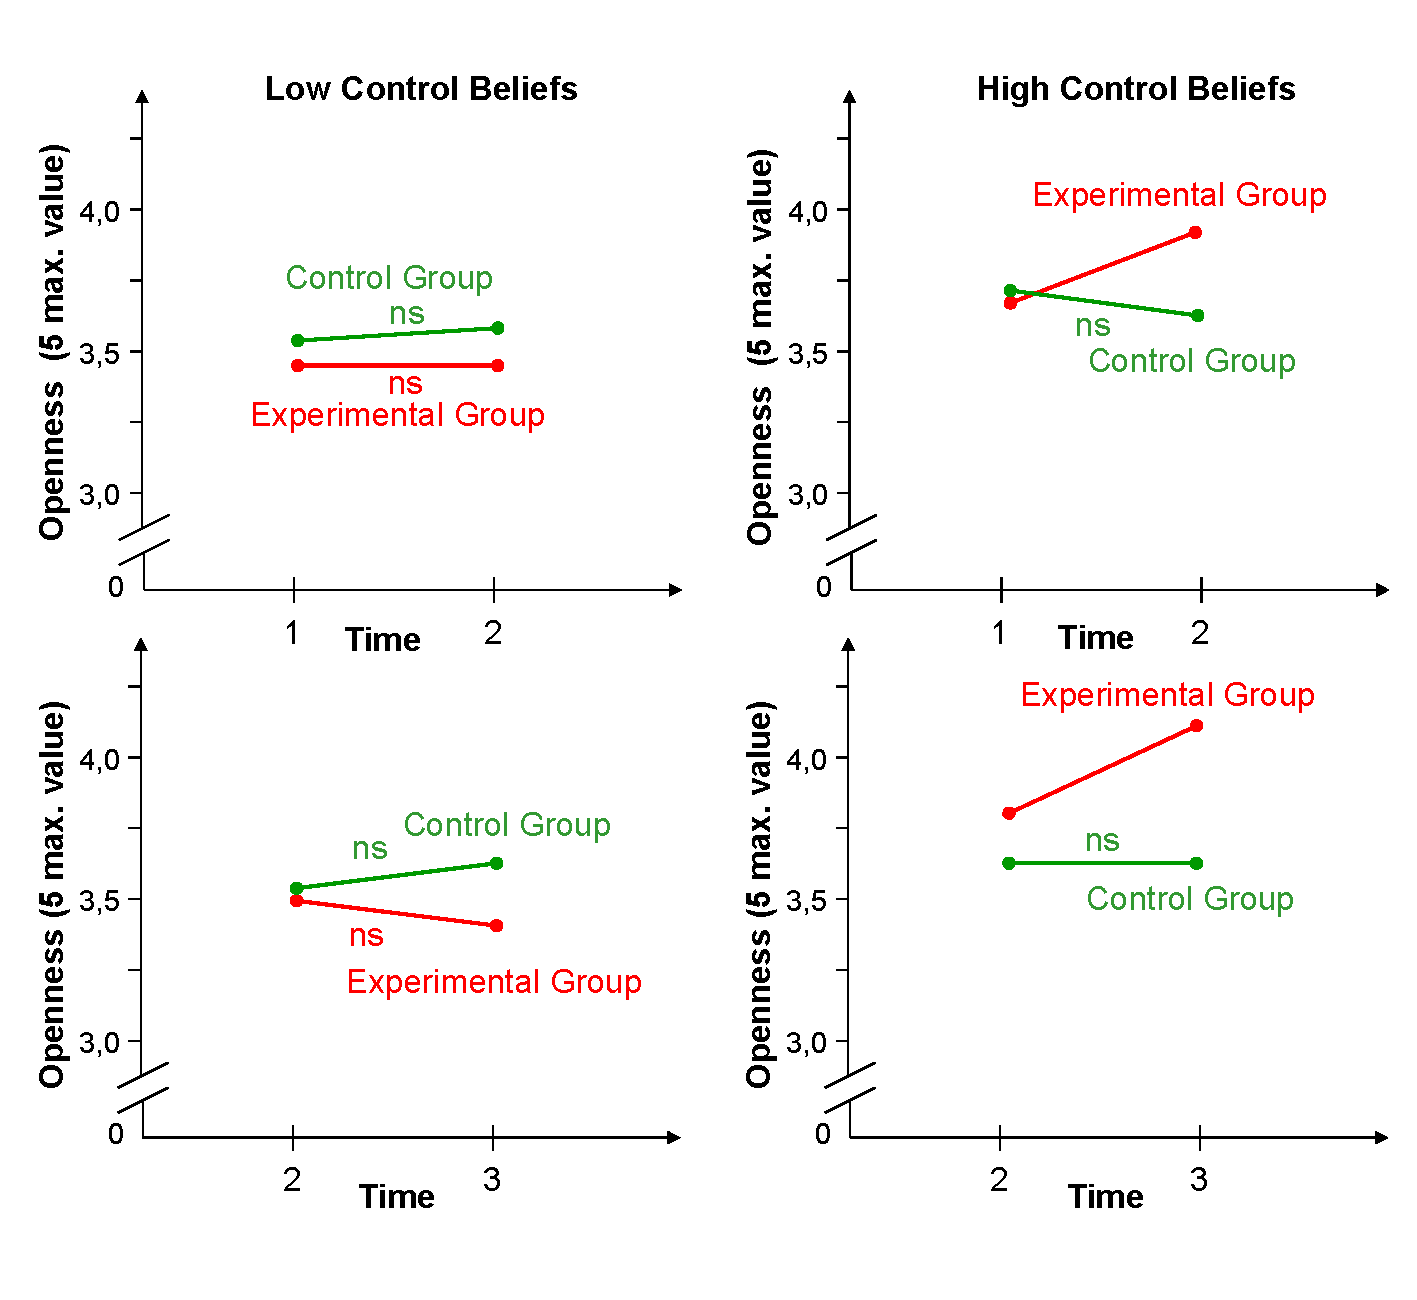
\includegraphics{profUrsulaStaudinger-fig3}}
    \caption{For participants with above median levels of internal control beliefs, the participation in the EFI program resulted in increases in Openness to Experiences. These increases were sustained across a period of 12 months (M\"uhlig-Versen \& Staudinger, in preparation).}
    \label{fig3:profUrsulaStaudinger}
  \end{center}
\end{figure}

\newpage

 All in all, the study shows that most likely it is not enough to become active to feel better but rather that specific circumstances, such as skill training and/or self-determination, need to be attended to as well.
 
\textit{The Effects of the Work Context on Adult Development}

 This is a new area of research that has started to emerge over the last year. One aspect that is of interest here is the effect of aging stereotypes present at the workplace on productivity and well being of older workers. First insights were gained from a JCLL pilot study that was conducted in the context of the Executive Master Program on Aging Workforce Management (LKI). In a sample of about 600 employees from 10 companies, we found as expected that older employees of companies with a rather negative aging stereotype showed poorer self-regulation as well as poorer job performance.


\paragraph{Collaborations}

\begin{itemize}
\item Deutsches Zentrum f\"ur Altersfragen DZA, Berlin\\ Prof. Dr. Clemens Tesch-R\"omer
\item Kassel University\\ Prof. Dr. Ekkehard Frieling 
\item Bremen University\\ Prof. Dr. Johannes Huinink
\item Yale University\\ Prof. Becca Levy, PhD
\end{itemize}

\begin{bibunit}[apalike]
\nocite{*}
\putbib[profUrsulaStaudinger3]
\end{bibunit}

\enlargethispage{2cm}
\paragraph{Grants}
\begin{itemize}
\item DFG STA 540/5 - 1/2 (PI: U.M. Staudinger): Age-heterogeneous interaction as facilitative developmental context (2003-2006).
\item BMFSFJ (PI: U.M. Staudinger): Personality development in old age: A natural intervention study (2001-2006).
\item Leopoldina (PI: U.M. Staudinger): Leotech Aging: Network that investigates Aging, Education and Work (2006-2009).
\item BMBF (PI: JCLL). U.M. Staudinger, U. Kunzmann: subproject ``Images of Aging'' within the joint research project ``Effects of Matches/Mismatches between Aspects of Human and Social Capital, Corporate Strategy and Work Organization on the Physical and Mental Well-Being of Employees''. 
\item DFG Travel Grant for Eva-Marie Kessler for Gerontological Society of America Annual Meeting 2006
\end{itemize}
